\documentclass[11pt]{article}
\usepackage[margin=1in]{geometry}
\usepackage{amsmath,mathtools,amssymb,amsthm,booktabs,tikz,array}
\usepackage[colorlinks=true,linkcolor=teal,urlcolor=teal,citecolor=teal]{hyperref}
\newtheorem{theorem}{Theorem}
\newtheorem{proposition}[theorem]{Proposition}
\newtheorem{corollary}[theorem]{Corollary}
\theoremstyle{remark}
\newtheorem{remark}[theorem]{Remark}
\newcommand{\R}{\mathbb R}
\newcommand{\E}{\mathbb E}
\newcommand{\norm}[1]{\left\lVert#1\right\rVert}
\newcommand{\Lam}{\Lambda}
\providecommand{\benchmarkExactRows}{%
tilt family, nine $(a,\beta)$ pairs & 0.01--0.05 & 1.89--1.98 & 1.0000 & 1.0000 & 3 & 0.02 \\
adverse family, $\varepsilon=1/2$, budget 64 & 1.00 & 64.00 & 1.0000 & 1.0163 & 63 & 0.06 \\
adverse family, $\varepsilon=1/2$, budget 256 & 1.00 & 64.00 & 1.0000 & 1.0011 & 255 & 0.28 \\
adverse family, $\varepsilon=1/10$, budget 64 & 1.00 & 1600 & 1.0000 & 1.0269 & 63 & 0.06 \\
adverse family, $\varepsilon=1/10$, budget 256 & 1.00 & 1600 & 1.0000 & 1.0012 & 255 & 0.28 \\
adverse family, $\varepsilon=1/100$, budget 64 & 1.00 & 160000 & 1.0000 & 1.0348 & 63 & 0.07 \\
adverse family, $\varepsilon=1/100$, budget 256 & 1.00 & 160000 & 1.0000 & 1.0014 & 255 & 0.31 \\
}

\providecommand{\benchmarkGenericRows}{%
$n=2$, $r=1/64$, three polygons & 0.74--1.00 & 1.00 & 1.00 & 14 & 0.10 \\
$n=2$, $r=1/16$, three polygons & 0.76--1.00 & 0.98--0.99 & 0.99--1.00 & 14 & 0.10 \\
$n=2$, $r=1/4$, three polygons & 0.86--1.00 & 0.90--0.97 & 0.95--1.00 & 10 & 0.09 \\
$n=3$, $r=1/64$, three polygons & 0.30--0.46 & 0.96--0.99 & 0.99--1.00 & 20 & 0.18 \\
$n=3$, $r=1/16$, three polygons & 0.32--0.49 & 0.87--0.94 & 0.97--0.99 & 23 & 0.21 \\
$n=3$, $r=1/4$, three polygons & 0.48--0.63 & 0.68--0.69 & 0.91--0.98 & 20 & 0.19 \\
$n=4$, $r=1/64$, three polygons & 0.19--0.70 & 0.98--0.99 & 1.00 & 57 & 0.63 \\
$n=4$, $r=1/16$, three polygons & 0.19--0.73 & 0.91--0.97 & 0.98--1.00 & 57 & 0.68 \\
$n=4$, $r=1/4$, three polygons & 0.21--0.86 & 0.72--0.86 & 0.93--1.00 & 47 & 0.59 \\
$n=6$, $r=1/64$, three polygons & 0.12--0.32 & 0.96--0.98 & 1.00 & 247 & 3.21 \\
$n=6$, $r=1/16$, three polygons & 0.13--0.34 & 0.86--0.94 & 0.99--1.00 & 243 & 3.40 \\
$n=6$, $r=1/4$, three polygons & 0.15--0.46 & 0.57--0.80 & 0.96--1.00 & 218 & 4.01 \\
$n=8$, $r=1/64$, three polygons & 0.15--0.28 & 0.95--0.98 & 1.00 & 679 & 2.84 \\
$n=8$, $r=1/16$, three polygons & 0.17--0.30 & 0.83--0.93 & 0.99--1.00 & 652 & 2.75 \\
$n=8$, $r=1/4$, three polygons & 0.26--0.42 & 0.56--0.75 & 0.96--1.00 & 407 & 1.88 \\
$n=4$, $r=1/16$, denominators $2^{8}$ & 0.56 & 0.93 & 0.99 & 71 & 0.65 \\
$n=4$, $r=1/16$, denominators $2^{20}$ & 0.46 & 0.93 & 0.99 & 101 & 1.17 \\
$n=4$ plus an inactive plane, $r=1/16$ & 0.66 & 0.95 & 0.99 & 93 & 1.15 \\
$n=4$ plus a near-coincident plane, $r=1/16$ & 0.66 & 0.94 & 0.99 & 168 & 1.80 \\
$n=8$, $r=1/4$, region cap 100 & -- & -- & -- & refused & -- \\
}

\title{Exact sensitivity certificates for planar transport maps\\[4pt]
\large Coefficient uncertainty, a convergent box refinement, and a sharp three-atom calibration}
\author{Anonymous}
\date{7 October 2026\quad Version 0.2.0\quad Unrefereed candidate}
\begin{document}
\maketitle
\begin{abstract}
An optimal transport map can change substantially even when its target measure
moves only a little. We give an exact-arithmetic certificate procedure for
finite affine-max transport maps on rational convex polygons. It computes the
map discrepancy, separately checks a primal--dual witness for target transport
cost, and bounds map discrepancy uniformly over an affine-coefficient box by a
possible-winner envelope that needs neither fixed cell combinatorics nor fixed
target masses. The envelope relaxes the problem in two distinct ways, and an
admissible two-plane family shows that its relative conservatism is unbounded:
the envelope is $4$ while the sharp maximum is $\varepsilon^2/4$. We prove that
the gap is nevertheless linear in the largest coefficient radius, with an
explicit constant, and derive from this a convergent box-subdivision refinement
that returns a certified interval $[\mathrm{LB},\mathrm{UB}]$ around the sharp
maximum, the lower bound being attained by an explicit realisation. A
two-parameter extension of an existing three-atom example gives closed formulas
for map error, target distance, and their difference, with a corner maximum on
admissible rectangles. A bounded synthetic benchmark compares the envelope with
the elementary slope-diameter bound, with explicit realisations, and with the
refinement. The contribution is a scoped certificate implementation with proved
tightness and convergence statements, not a new general transport-stability
exponent.
\end{abstract}

\section{Problem and relationship to prior work}
Let $K\subset\R^2$ be a bounded convex polygon with positive area, and let
$\rho=|K|^{-1}1_K\,dx$. Consider potentials
\[
 u(x)=\max_{1\leq i\leq m}(a_i\cdot x+c_i),\qquad
 v(x)=\max_{1\leq j\leq n}(b_j\cdot x+d_j).
\]
Within each potential, repeated slopes can be merged by retaining the largest
intercept. Write $T_u=\nabla u$, $T_v=\nabla v$ almost everywhere and
$\mu=(T_u)_\#\rho$, $\nu=(T_v)_\#\rho$. Our primary quantities are
\[
 F(u,v)=\norm{T_u-T_v}_{L^2(\rho)}^2,
 \qquad W_2(\mu,\nu)^2.
\]
They are different: the common-source coupling yields $W_2^2\leq F$, but it
need not be optimal between the targets.

The $L^2$ distance between optimal maps from a fixed source is the Monge
embedding of M\'erigot, Delalande and Chazal \cite{MDC}, who relate it to
$W_2$ and, in their supplementary Lemma~5.1, show with two equal-mass atoms
rotating on a circle that the map can move like the square root of the
target distance even when every atom keeps a fixed positive mass. Delalande
and M\'erigot \cite{DM} prove quantitative stability for a fixed source and a
varying target, with exponent $1/6$ in the compact convex case; Letrouit
\cite{Let} shows that for a uniform source on a suitable bounded open set no
exponent above $1/3$ is possible and conjectures $1/2$ for convex sources.
Divol, Niles-Weed and Pooladian \cite{DNP} obtain semi-discrete map stability
of order $W_2^{1/3}$ for discrete targets that may have different supports,
with constants depending on the masses and the geometry of the atoms. Bansil
and Kitagawa \cite{BK} give quantitative stability of the cells when masses
change on a fixed site set, without a lower bound on individual masses. An,
Lei and Gu \cite{ALG} use the intersections of two source-cell decompositions
to construct a target coupling and note that it need not be optimal. Carlier,
Delalande and M\'erigot \cite{CDM} study the different problem of a fixed map
and a varying source. Reduced-order optimal-value estimators \cite{BN} are
another distinct certification problem. Possible-winner regions built from
upper and lower envelopes of the competing values have a close antecedent in
the uncertain Voronoi diagrams of Xie et al.\ \cite{Xie}, whose partitions
record the set of objects that can be nearest to each region; our envelope
applies the same screening principle to affine coefficients and integrates a
transport cost over it. The scalar function $H$ of Section~\ref{sec:tilt} is a
shifted and scaled Huber penalty, the uniform smoothing of the absolute value
\cite{RQS}; its transport role is what is used here.

Our starting calibration comes from OpenAI's three-affine-max construction
\cite{OAI}, which Letrouit's instability result motivates. We retain its
attribution. The calculations below extend that example by allowing both a
change of central mass and a tilt, and turn it into a sharp uncertainty test.
We do not use or independently validate the source's claimed general one-third
upper bound. The bounded prior-art search is documented in the accompanying
package; historical priority for the specialised formulas and envelope is not
asserted. Table~\ref{tab:compare} positions the certificate.

\begin{table}[tbp]
\centering\small
\begin{tabular}{@{}>{\raggedright}p{2.6cm}>{\raggedright}p{2.6cm}>{\raggedright}p{2.6cm}>{\raggedright}p{2.6cm}p{3.6cm}@{}}
\toprule
Work & What varies & What is controlled & Degeneracies allowed & Quantity certified or bounded\\
\midrule
M\'erigot et al.\ \cite{MDC}; Delalande--M\'erigot \cite{DM} & target measure & source density, compact support & general targets & $\norm{T_\mu-T_\nu}_{L^2}$ by a power of $W_p(\mu,\nu)$\\
Divol et al.\ \cite{DNP} & discrete target, possibly different support & masses, separation, count of atoms & none below the stated lower bounds & $\norm{T_\mu-T_\nu}_{L^2}\lesssim W_2^{1/3}$\\
Bansil--Kitagawa \cite{BK} & target masses on fixed sites & site set & zero masses & summed symmetric cell differences by $\ell^1$ mass change\\
An--Lei--Gu \cite{ALG} & two maps, common source & auxiliary density & -- & overlay coupling (may be non-optimal)\\
Xie et al.\ \cite{Xie} & uncertain point sites & distance bounds & -- & possible nearest-neighbour sets\\
This note & affine coefficients in a box & reference potential, polygon & disappearing cells, changing masses, coincident planes & exact $F$, witnessed $W_2^2$, envelope $B\ge\sup F$, interval $[\mathrm{LB},\mathrm{UB}]\ni\sup F$\\
\bottomrule
\end{tabular}
\caption{What varies, what is controlled, and what is certified. The entries for other works are summaries of their stated settings, not reproductions of their theorems.}
\label{tab:compare}
\end{table}

\section{Exact map and target certificates}
Let $C_i$ and $D_j$ be the maximizing cells of $u$ and $v$. Ties between
distinct slopes lie on finitely many lines, so these cells partition $K$
up to null sets.

\begin{proposition}[Optimality and exact overlay]\label{prop:overlay}
The map $T_u$ is the unique quadratic optimal map from $\rho$ to $\mu$.
The matrix $Q_{ij}=|C_i\cap D_j|/|K|$ has the target masses as its row and
column sums, and
\begin{equation}\label{eq:overlay}
 F(u,v)=\sum_{i,j}Q_{ij}|a_i-b_j|^2.
\end{equation}
For rational input coefficients and polygon vertices, all quantities in
\eqref{eq:overlay} are rational and computable by polygon clipping.
\end{proposition}
\begin{proof}
For any coupling $\pi$ of $\rho$ and $\mu$,
\[
 \int x\cdot y\,d\pi\leq\int u\,d\rho-\sum_i c_i\mu(\{a_i\}).
\]
The graph coupling of $T_u$ attains equality. Maximizing this scalar product
minimizes quadratic cost because the marginal second moments are fixed.
Equality forces the maximizing slope, unique almost everywhere, which proves
uniqueness. Equation~\eqref{eq:overlay} follows by integrating its constant
integrand on each overlay cell. Rational half-plane intersections have
rational vertices, and the shoelace area formula preserves rationality.
\end{proof}

We check target optimality separately. Given a nonnegative matrix $P$ with
the prescribed target marginal sums and vectors $\alpha,\beta$, require
\begin{equation}\label{eq:dual}
 \alpha_i+\beta_j\leq |a_i-b_j|^2,\qquad
 \sum_{i,j}P_{ij}|a_i-b_j|^2
 =\sum_i\mu_i\alpha_i+\sum_j\nu_j\beta_j.
\end{equation}
Weak duality then proves that the displayed cost equals $W_2^2$. The checker
uses exact equalities and inequalities, rather than an optimizer's status.
It rejects a feasible but nonoptimal coupling when the equality fails.

\section{A coefficient-box uncertainty certificate}\label{sec:box}
Fix $u$. For each $j$, let the two slope coordinates and intercept of the
comparison potential vary independently around $(b_j,d_j)$ with radii
$(r_{j1},r_{j2},r_{j0})\geq0$. Define
\begin{align*}
 e_j(x)&=r_{j1}|x_1|+r_{j2}|x_2|+r_{j0},\\
 U_j(x)&=b_j\cdot x+d_j+e_j(x),\qquad
 L_j(x)=b_j\cdot x+d_j-e_j(x),\\
 J(x)&=\{j:U_j(x)\geq L_k(x)\text{ for every }k\},\\
 M_{ij}&=\sum_{\ell=1}^2(|a_{i\ell}-b_{j\ell}|+r_{j\ell})^2.
\end{align*}

\begin{theorem}[Uniform map-error enclosure]\label{thm:box}
For every single global realization $\widetilde v$ of the coefficient box,
\begin{equation}\label{eq:box}
 F(u,\widetilde v)\leq
 B:=\frac1{|K|}\sum_i\int_{C_i}\max_{j\in J(x)}M_{ij}\,dx.
\end{equation}
For rational box data, $B$ is exactly computable by a finite arrangement of
lines and rational polygon areas. No preservation of cell combinatorics,
positive individual cell masses, or fixed target masses is assumed.
\end{theorem}
\begin{proof}
If $j$ wins at $x$ for a realization, then its realized value is at most
$U_j(x)$, while every competing realized value is at least $L_k(x)$.
Thus $j\in J(x)$. The coordinatewise triangle inequality bounds the
squared slope discrepancy by $M_{ij}$ on $C_i$, proving the pointwise
inequality and then \eqref{eq:box}.

On any coordinate orthant, each $U_j-L_k$ is affine. Partition each
$C_i$ intersected with that orthant by their zero lines. The set $J(x)$
is constant on the interior of each positive-area piece; its contribution
is that piece's rational area times a rational constant. Boundaries are
null. Identically zero comparisons cause no split. For any fixed
realization, coincident affine functions have identical slopes; ties
between unequal slopes remain null. These degeneracies do not invalidate
the integral.
\end{proof}

Three elementary consequences are used by the implementation: $J(x)$ is never
empty, because a nominal maximiser $j$ satisfies $U_j\ge b_j\cdot x+d_j\ge
b_k\cdot x+d_k\ge L_k$; with all radii zero, $B$ equals the exact discrepancy
$F(u,v)$ almost everywhere; and the arithmetic mean of the vertices of a
positive-area convex polygon lies in its interior, so it is a valid sign
representative for each arrangement region. We also record the elementary
slope-diameter bound
\begin{equation}\label{eq:baseline}
 B_0:=\sum_i\rho(C_i)\max_j M_{ij}\ \ge\ B,
\end{equation}
which ignores the winner screening; the benchmark of Section~\ref{sec:bench}
measures what the screening buys.

\subsection{Two relaxations, and an adverse family}
The envelope relaxes the problem in two distinct ways. First, $M_{ij}$
maximises the slope discrepancy of plane $j$ over the whole box without
requiring that the same coefficient choice makes $j$ win at $x$. Second, the
pointwise maximum lets different source points use different global
parameters. The following family, supplied by the external review of version
0.1.0 and rederived here, shows that the first relaxation costs an unbounded
factor while the second costs exactly a further factor two.

\begin{proposition}[Adverse family]\label{prop:loose}
Let $K=[1,2]\times[0,1]$, $u(x)=x_1$, and let the comparison box consist of
the fixed plane $x_1$ and the plane $bx_1+\varepsilon$ with nominal $b=0$,
slope radius $1$ in the first coordinate and all other radii zero, where
$0\le\varepsilon\le1$ is rational. A realisation is
$v_b(x)=\max\{x_1,\,bx_1+\varepsilon\}$ with one global $b\in[-1,1]$. Put
$d=1-b\in[0,2]$. Then
\begin{equation}\label{eq:looseF}
 F(u,v_b)=\begin{cases}d^2,&0\le d\le\varepsilon/2,\\
 \varepsilon d-d^2,&\varepsilon/2\le d\le\varepsilon,\\
 0,&d\ge\varepsilon,\end{cases}
 \qquad
 \sup_{b\in[-1,1]}F(u,v_b)=\frac{\varepsilon^2}{4},
\end{equation}
the supremum being attained only at the interior parameter $b=1-\varepsilon/2$
when $\varepsilon>0$, while both endpoints $b=\pm1$ give $F=0$. The envelope
of Theorem~\ref{thm:box} and the baseline \eqref{eq:baseline} both equal $4$
for every such $\varepsilon$, with a single arrangement region. The pointwise
supremum that respects winner--slope compatibility but still lets $b$ depend
on $x$ integrates to $\varepsilon^2/2$. Hence
\[
 \frac{\varepsilon^2}{4}=\sup_b F(u,v_b)\ \le\ \frac{\varepsilon^2}{2}\ \le\ 4=B,
\]
the first inequality costs exactly a factor $2$ in this family and the second a
factor $8/\varepsilon^2$, so the envelope-to-maximum ratio $16/\varepsilon^2$ is
unbounded with the slope radius fixed, and at $\varepsilon=0$ every realisation
has $F=0$ while $B=4$.
\end{proposition}
\begin{proof}
Plane $2$ wins where $dx_1<\varepsilon$. For $d>0$ its cell is
$\{1\le x_1<\min(2,\varepsilon/d)\}\times[0,1]$, of mass
$(\min(2,\varepsilon/d)-1)_+$ since $|K|=1$, and its squared slope
discrepancy is $(1-b)^2=d^2$, which gives \eqref{eq:looseF}; at $d=0$ the
plane has the reference slope and $F=0$ after merging. The branch $d^2$
increases on $[0,\varepsilon/2]$ and $\varepsilon d-d^2$ decreases on
$[\varepsilon/2,\varepsilon]$, so the supremum is $\varepsilon^2/4$ at
$d=\varepsilon/2$. For every $x\in K$, $U_2(x)=x_1+\varepsilon\ge x_1=L_1(x)$,
so $2\in J(x)$ everywhere; $M_{12}=(1+1)^2=4$ and $M_{11}=0$, so the integrand
is $4$ everywhere, and $B_0=4$ likewise. At a point with $x_1\in(1,2)$, plane
$2$ wins exactly for $b>1-\varepsilon/x_1$, and the supremum of $(1-b)^2$ over
these $b$ is $(\varepsilon/x_1)^2$; integrating,
$\varepsilon^2\int_1^2x_1^{-2}\,dx_1=\varepsilon^2/2$.
\end{proof}

The family also shows that the corner reduction of
Corollary~\ref{cor:corner} below cannot extend to general coefficient boxes:
both endpoints give error zero while an interior parameter gives the maximum.
The loss is unrelated to computational scale, since one region suffices. It is
a limitation of informativeness, not a counterexample to Theorem~\ref{thm:box}.

\subsection{Tightness at small radius}
Let $r$ be the largest radius entry, $v$ the nominal realisation (duplicate
slopes merged, largest intercept kept; in the proof the nominal winner at a
point is an original index with the winning slope and the largest intercept,
so that $J$, $M_{ij}$ and the pair count use original indices),
$R_K=\max_{x\in K}(|x_1|+|x_2|+1)$,
$D_K$ any upper bound for the Euclidean diameter of $K$ (the implementation
uses the $\ell^1$ vertex diameter), and
\[
 \Lam=\max_{i,j}\sum_{\ell=1}^2\big(|a_{i\ell}-b_{j\ell}|+r_{j\ell}\big),
\]
an $\ell^1$ bound for the distance between any reference slope and any
realised comparison slope. Norms of slopes are Euclidean.

\begin{theorem}[Tightness]\label{thm:tight}
\begin{equation}\label{eq:gamma}
 0\ \le\ B-F(u,v)\ \le\ \gamma(r):=2r\Lam+2r^2+\frac{4rR_KD_K\,n(n-1)\Lam}{|K|}.
\end{equation}
\end{theorem}
\begin{proof}
The lower inequality is Theorem~\ref{thm:box} for the nominal realisation. Fix
$x$ in the interior of some $C_i$, off every nominal tie line, and let $k$ be
the nominal winner at $x$. For $j\in J(x)$ write
\[
 M_{ij}-|a_i-b_k|^2=\big(M_{ij}-|a_i-b_j|^2\big)+\big(|a_i-b_j|^2-|a_i-b_k|^2\big).
\]
The first bracket equals $\sum_\ell(2r_{j\ell}|a_{i\ell}-b_{j\ell}|+r_{j\ell}^2)
\le2r\Lam+2r^2$. The second vanishes for $j=k$. For $j\ne k$ in $J(x)$, the
membership $U_j(x)\ge L_k(x)$ gives $g_k(x)-g_j(x)\le e_j(x)+e_k(x)\le2rR_K$,
where $g_j=b_j\cdot x+d_j$, and $g_k(x)\ge g_j(x)$ because $k$ wins; so $x$
lies in $T_{jk}:=\{y\in K:0\le g_k(y)-g_j(y)\le2rR_K\}$. Moreover
$|a_i-b_j|^2-|a_i-b_k|^2=(b_k-b_j)\cdot(2a_i-b_j-b_k)\le2\Lam|b_k-b_j|$,
since a Euclidean norm is at most the $\ell^1$ norm bounded by $\Lam$.
Integrating over $K$,
\[
 |K|\big(B-F(u,v)\big)\le(2r\Lam+2r^2)|K|+\sum_{j\ne k}|T_{jk}|\,2\Lam|b_k-b_j|.
\]
A pair with $b_j=b_k$ contributes nothing. Otherwise $T_{jk}$ lies in a closed
strip of width $2rR_K/|b_k-b_j|$, and a strip of width $w$ meets a convex set
of diameter at most $D_K$ in area at most $wD_K$ (integrate the chord lengths
across the strip). Each ordered pair therefore contributes at most
$4rR_KD_K\Lam$, and there are at most $n(n-1)$ of them.
\end{proof}

\begin{remark}[Margins and slope separation]\label{rem:margin}
Let $\mu(x)$ be the nominal margin: the winning value minus the largest
competing value among planes with a different slope. Where $\mu(x)>2rR_K$,
$J(x)$ contains only planes with the winner's slope and the excess is at most
$2r\Lam+2r^2$; elsewhere it is at most $\max_{i,j}M_{ij}$. Hence
$B-F(u,v)\le2r\Lam+2r^2+(\max_{i,j}M_{ij})\,|\{\mu\le2rR_K\}|/|K|$, and the
strip bound gives $|\{\mu\le t\}|\le n(n-1)D_Kt/\sigma$ with $\sigma$ the
smallest distance between distinct comparison slopes. The uniform constant in
\eqref{eq:gamma} avoids $\sigma$ because the strip width and the cost
difference are reciprocal in $|b_k-b_j|$. With the $\ell^1$ vertex diameter as
$D_K$, all quantities in $\gamma$ are rational for rational data; the test suite
checks \eqref{eq:gamma} on $108$ random boxes.
\end{remark}

\subsection{A convergent refinement}
Theorem~\ref{thm:box} applies to every sub-box of the coefficient box, and
Theorem~\ref{thm:tight} says that the envelope of a sub-box of radius $r$
overshoots the exact error at its centre by $O(r)$. This gives a certificate
that retains the global parameter dependence.

\begin{theorem}[Convergent box subdivision]\label{thm:refine}
Let the coefficient box be covered by finitely many sub-boxes $P$ of the same
form, with largest radius $r_*$. Put $\mathrm{UB}=\max_PB(P)$ and let
$\mathrm{LB}$ be the largest value of $F(u,\cdot)$ over any finite set of
realisations in the box that contains every sub-box centre $c(P)$. Then
\[
 \mathrm{LB}\ \le\ \sup_{\widetilde v}F(u,\widetilde v)\ \le\ \mathrm{UB},
 \qquad
 \mathrm{UB}-\mathrm{LB}\le\max_P\big[B(P)-F(u,v_{c(P)})\big]\le\gamma_{\mathrm{box}}(r_*),
\]
where $\gamma_{\mathrm{box}}$ is \eqref{eq:gamma} with $\Lam$ computed for the
full box.
\end{theorem}
\begin{proof}
Every realisation lies in some $P$, so Theorem~\ref{thm:box} for that sub-box
gives $F\le B(P)\le\mathrm{UB}$; $\mathrm{LB}$ is a maximum of feasible values.
For the gap, $\mathrm{UB}-\mathrm{LB}\le B(P^*)-F(u,v_{c(P^*)})$ for a sub-box
$P^*$ attaining $\mathrm{UB}$, and Theorem~\ref{thm:tight} applies to $P^*$
with its own constant, which is at most $\gamma_{\mathrm{box}}$ because for a
sub-interval $[b'-r',b'+r']$ of $[b-r,b+r]$ one has
$|a-b'|+r'\le|a-b|+|b-b'|+r'\le|a-b|+r$.
\end{proof}

The implementation (\texttt{refine\_bound}) keeps a best-first heap of
sub-boxes ordered by their envelopes, splits the sub-box with the largest
envelope along its widest coordinate, evaluates the exact $F$ at each child
centre and at the child's outer endpoint along the split coordinate (literal
points of the box, which supply $\mathrm{LB}$; the attaining point is returned
both as coefficients and as its merged equivalent), and
never splits a sub-box whose envelope is at most $\mathrm{LB}$; pruning
preserves both inequalities because such sub-boxes cannot exceed
$\mathrm{LB}$. It stops when the largest remaining envelope is at most
$\mathrm{LB}$, when $\mathrm{UB}-\mathrm{LB}$ is within a requested tolerance,
or when the box budget is exhausted; in every case it returns the valid
interval, the number of sub-boxes evaluated and the stop reason. Splitting the
widest coordinate halves the largest radius of a lineage at least once every
$3n$ splits, so for any positive tolerance only finitely many sub-boxes can
remain above it and the loop terminates; exact convergence occurs only when a
probe meets a maximiser, which bisection from $[-1,1]$ never does at the
non-dyadic maximiser $b=19/20$ of the adverse family. Uniform refinement needs a number of
sub-boxes exponential in the box dimension $3n$; the benchmark records the
consequence. On the adverse family the interval reaches
$[\varepsilon^2/4\cdot(1-10^{-5}),\,\varepsilon^2/4\cdot(1+1.4\cdot10^{-3})]$
with $256$ sub-boxes, where the envelope was $4$.

\section{A sharp two-parameter calibration}\label{sec:tilt}
Let $d\geq2$, let $\rho$ be uniform on $[-1,1]^d$, and assume
\begin{equation}\label{eq:admissible}
 0<a<1,\qquad 0<a+s-|b|,\qquad a+s+|b|<1.
\end{equation}
Define
\[
 u_a(x)=\max\{-x_1,x_1,a\},\quad
 v_{a,s,b}(x)=\max\{-x_1,x_1,a+s+bx_2\}.
\]
The central strips have slice half-widths $a$ and $a+s+bt$ at $x_2=t$.
Their target laws are
\begin{align*}
 \mu_a&=\tfrac{1-a}{2}(\delta_{-e_1}+\delta_{e_1})+a\delta_0,\\
 \nu_{a,s,b}&=\tfrac{1-a-s}{2}(\delta_{-e_1}+\delta_{e_1})+(a+s)\delta_{be_2}.
\end{align*}

\begin{theorem}[Exact error and coupling excess]\label{thm:tilt}
Under \eqref{eq:admissible}, set
\[
 H(s,b)=\begin{cases}|s|,& |s|\geq|b|,\\
 (s^2+b^2)/(2|b|),& |s|<|b|.
 \end{cases}
\]
Then
\begin{align}
 F(u_a,v_{a,s,b})&=H(s,b)+(a+s)b^2,\label{eq:F}\\
 W_2(\mu_a,\nu_{a,s,b})^2&=|s|+(a+s)b^2.\label{eq:W}
\end{align}
In particular the overlap coupling is target-optimal exactly when
$|s|\geq|b|$. Its excess cost is
\begin{equation}\label{eq:gap}
 F-W_2^2=\begin{cases}0,& |s|\geq|b|,\\
 (|b|-|s|)^2/(2|b|),& |s|<|b|.
 \end{cases}
\end{equation}
\end{theorem}
\begin{proof}
The central intervals are nested on each slice. Their symmetric difference
has conditional source probability $|s+bt|$. The first-coordinate squared
map difference is the indicator of that symmetric difference; the
second-coordinate contribution is $b^2$ on the new central strip.
Consequently $F=\E|s+bU|+(a+s)b^2$, with $U$ uniform on $[-1,1]$.
Integrating the absolute value, splitting at $-s/b$ when it is internal,
gives $H$ and \eqref{eq:F}. (For $|b|>0$, $H(s,b)=h_{|b|}(s)/|b|+|b|/2$ with
$h_\lambda$ the Huber penalty \cite{RQS}.)

Order the atoms (left, centre, right), so that the cost matrix is
$\begin{psmallmatrix}0&1+b^2&4\\1&b^2&1\\4&1+b^2&0\end{psmallmatrix}$.
For $s\geq0$ the coupling keeps the common mass on each atom pair, namely
$\frac{1-a-s}{2}$ on left$\to$left, $a$ on centre$\to$centre (the centre moves
from $0$ to $be_2$, cost $b^2$), $\frac{1-a-s}{2}$ on right$\to$right, and
moves $s/2$ from each outer atom to the new centre at cost $1+b^2$ each. For
$s<0$ it keeps $\frac{1-a}{2}$, $a+s$, $\frac{1-a}{2}$ on the diagonal and
moves $-s/2$ from the old centre to each outer atom at cost $1$ each.
Horizontal cost is $|s|$ and vertical cost is $(a+s)b^2$. Exact feasible
duals in \eqref{eq:dual} are
\[
\begin{array}{c|cc}
 &\alpha&\beta\\\hline
 s\geq0&(1,0,1)&(-1,b^2,-1)\\
 s<0&(-1,0,-1)&(1,b^2,1).
\end{array}
\]
Their objective equals the constructed cost, proving \eqref{eq:W}.
Subtracting gives \eqref{eq:gap}, including $s=b=0$. Coordinates beyond
the first two integrate out.
\end{proof}

\begin{figure}[tbp]
\centering
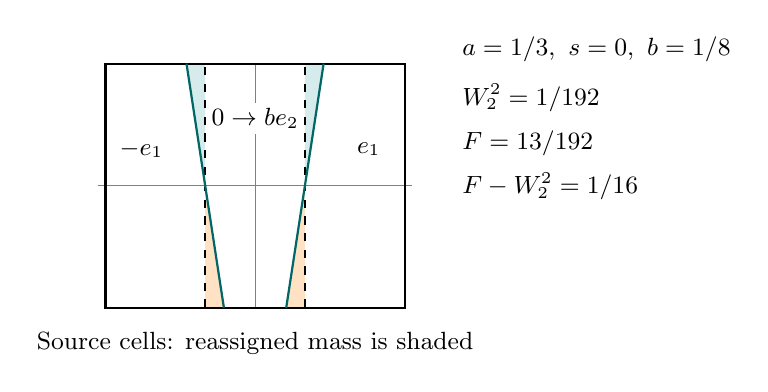
\begin{tikzpicture}[x=1.9cm,y=1.55cm,font=\small]
\fill[teal!16] (-.3333,0)--(-.4583,1)--(-.3333,1)--cycle;
\fill[teal!16] (.3333,0)--(.4583,1)--(.3333,1)--cycle;
\fill[orange!23] (-.3333,0)--(-.2083,-1)--(-.3333,-1)--cycle;
\fill[orange!23] (.3333,0)--(.2083,-1)--(.3333,-1)--cycle;
\draw[gray] (-1.05,0)--(1.05,0);
\draw[gray] (0,-1)--(0,1);
\draw[thick] (-1,-1) rectangle (1,1);
\draw[dashed,thick] (-.3333,-1)--(-.3333,1);
\draw[dashed,thick] (.3333,-1)--(.3333,1);
\draw[teal!80!black,thick] (-.2083,-1)--(-.4583,1);
\draw[teal!80!black,thick] (.2083,-1)--(.4583,1);
\node[fill=white,inner sep=2pt] at (-.76,.3) {$-e_1$};
\node[fill=white,inner sep=2pt] at (.76,.3) {$e_1$};
\node[fill=white,inner sep=2pt] at (0,.55) {$0\to be_2$};
\node[below] at (0,-1.12) {Source cells: reassigned mass is shaded};
\node[anchor=west,align=left] at (1.32,.55) {$a=1/3,\ s=0,\ b=1/8$\\[7pt]
$W_2^2=1/192$\\[5pt]$F=13/192$\\[5pt]$F-W_2^2=1/16$};
\end{tikzpicture}
\caption{The targets have unchanged atom masses, yet their maps disagree on
source strips. Dashed boundaries belong to the reference map; solid boundaries
to the tilted map. Labels denote map values, not target points in the source
plane. Diagram coordinates are rounded for display; all reported values are exact.}
\end{figure}

\begin{corollary}[Sharp parameter-rectangle maximum]\label{cor:corner}
Fix $a$ and a closed rectangle $[s_-,s_+]\times[b_-,b_+]$ satisfying
\eqref{eq:admissible} throughout. The maximum of $F$ is the largest of its
four corner values. It is enough to check admissibility at the corners.
\end{corollary}
\begin{proof}
For fixed $b$, $\E|s+bU|$ is convex in $s$, and $(a+s)b^2$ is affine.
For fixed $s$, the first term is convex in $b$ and the second is convex
because $a+s>0$. Maximizing in the two coordinates successively reduces
the rectangle to its corners. Joint convexity is not required. The
admissibility margins $a+s-|b|$ and $1-a-s-|b|$ take their minima over
the rectangle at corners as well.
\end{proof}

For $s=0$, $b\in[-\beta,\beta]$, and $0<\beta<\min(a,1-a)$, the exact maximum
is $\beta/2+a\beta^2$. The envelope of Theorem~\ref{thm:box}, applied with
only the central vertical slope uncertain, is $\beta+a\beta^2$: the inner
ambiguous source strips have total mass $\beta/2$ and worst squared cost one;
the outer ambiguous strips have mass $\beta/2$ and cost $1+\beta^2$; the common
central region has mass $a-\beta/2$ and cost $\beta^2$. The gap $\beta/2$ is
the price of the pointwise relaxation in this family; the pointwise maxima are
attainable on each region, so the winner--slope relaxation costs nothing here,
in contrast with Proposition~\ref{prop:loose}. The refinement of
Theorem~\ref{thm:refine} closes the gap with three sub-boxes, because the
endpoint probes meet the corner maximum.

Setting $s=0$, $b=a/2$ and $0<a<1/2$ recovers the source's degenerating-mass
example \cite{OAI}: $W_2=a^{3/2}/2$ and $\sqrt F=\sqrt{a(1+a^2)}/2$.
Keeping $a$ fixed instead gives $W_2=\sqrt a\,|b|$ and
$\sqrt F\sim\sqrt{|b|/2}$. Thus even with fixed positive atom masses,
this family has square-root rather than Lipschitz map sensitivity as the
central site moves; the phenomenon itself is already in \cite{MDC}
(supplementary Lemma~5.1, two rotating atoms). These statements are direct
consequences of the calibration, not new general upper bounds.

\section{A bounded benchmark}\label{sec:bench}
Table~\ref{tab:exact} and Table~\ref{tab:generic} summarise the $65$ cases
recorded in \texttt{evidence/benchmark.json}, computed by the shipped
\texttt{benchmark.py} on one machine (Python~3.14, Apple~M2; process peak
memory $23$~MB; every exact field is recomputed and compared by its
\texttt{--check} mode). The families are: the tilt calibration with nine
$(a,\beta)$ pairs, where the exact maximum is known; the adverse family of
Proposition~\ref{prop:loose} for three $\varepsilon$; and generic random
rational potentials with $n\in\{2,3,4,6,8\}$ comparison planes, $n$ reference
planes, all $3n$ coefficients uncertain with a common radius
$r\in\{1/64,1/16,1/4\}$, on a square, a triangle and a pentagon, plus cases
with dyadic denominators $2^8$ and $2^{20}$, an inactive plane, a
near-coincident plane, and a region-cap refusal. The refinement budget is
$32$ sub-boxes for $n\le6$ and $8$ for $n=8$.

\begin{table}[tbp]
\centering\small
\begin{tabular}{@{}lcccccc@{}}
\toprule
Family & $B/B_0$ & $B/\sup F$ & $\mathrm{LB}/\sup F$ & $\mathrm{UB}/\sup F$ & boxes & s\\
\midrule
\benchmarkExactRows
\bottomrule
\end{tabular}
\caption{Families with a known sharp maximum. $B$ is the envelope, $B_0$ the slope-diameter bound \eqref{eq:baseline}, $[\mathrm{LB},\mathrm{UB}]$ the refinement interval at the stated budget; ranges are over the cases in the row. Wall time is the envelope plus the refinement.}
\label{tab:exact}
\end{table}

\begin{table}[tbp]
\centering\small
\begin{tabular}{@{}lccccc@{}}
\toprule
Cases & $B/B_0$ & $\mathrm{LB}/B$ & $\mathrm{UB}/B$ & regions & s\\
\midrule
\benchmarkGenericRows
\bottomrule
\end{tabular}
\caption{Generic random boxes with all $3n$ coefficients uncertain. $\mathrm{LB}$ is the largest exact error among the explicit realisations probed by the refinement; $\mathrm{UB}$ its refined envelope at the budget; regions is the largest arrangement size of the envelope; s the largest wall time in the row.}
\label{tab:generic}
\end{table}

Three observations are supported. First, the winner screening is what makes
the envelope informative: $B/B_0$ falls from $0.74$--$1.00$ at $n=2$ to
$0.12$--$0.46$ at $n=6$ and $0.15$--$0.42$ at $n=8$. Second, at small radius
the envelope is nearly attained: at $r=1/64$ explicit realisations reach
$0.95$--$1.00$ of $B$, at $r=1/16$ $0.83$--$0.99$, and at $r=1/4$
$0.56$--$0.97$, in line with the linear-in-$r$ statement of
Theorem~\ref{thm:tight}; the inactive plane, the near-coincident plane and
the long denominators change the region count, not the tightness. Third,
subdivision is decisive on low-dimensional boxes (the one-parameter tilt and
adverse families converge within three and $256$ sub-boxes) and marginal at
a budget of $32$ on $3n$-dimensional boxes, where halving one coordinate
barely changes the envelope; this is the exponential cost predicted after
Theorem~\ref{thm:refine}, and the certified lower bound is then the useful
output. The largest envelope took $0.52$~s with $679$ regions; the region cap
refuses rather than returning a partial sum. These are single-machine
observations, not performance claims.

\section{Implementation, checks, and limitations}
The accompanying Python implementation uses only the standard library and
exact rational arithmetic. Input floats, malformed rational strings such as
\texttt{1/0}, repeated reference slopes, invalid polygons, invalid marginal
sums, infeasible duals, and nonzero primal--dual gaps are rejected with a
diagnostic. Repeated slopes are merged explicitly by \texttt{merge\_planes}
before overlay. The uncertainty routines permit coinciding comparison planes
and disappearing cells. The envelope remains an upper bound, not necessarily
a realizable maximum; the refinement returns a certified interval whose lower
end is realised.

Tests compare the clipping implementation with a separately implemented
half-plane vertex-enumeration and convex-hull calculation. They cover $45$
exact calibration cases, $24$ generic polygon/potential pairs, invariances,
zero-radius exactness, the sharp-versus-enclosed uncertainty gap, a
$169$-point rectangle grid, the adverse family on a $101$-point grid for four
values of $\varepsilon$, the tightness inequality \eqref{eq:gamma} on $108$
random boxes, the monotone convergence and feasibility of the refinement, and
the rejection of malformed inputs. Thirty-two sampled box realizations provide
additional falsification tests, not proof of a uniform bound. Semantic
negative controls include a feasible nonoptimal overlap coupling and
corrupted primal or dual witnesses. The test suite runs in normal and
optimized Python modes; it does not rely on removable assertions. The
command-line \texttt{--check} mode recomputes every recorded field with the
same implementation: it is a reproducibility check, not an independent
verification.

The mathematical claims rest on the proofs above, while tests support the
implementation. Neither is formal proof-assistant verification or external
peer review. Version 0.1.0 of this note, which lacked
Propositions~\ref{prop:loose}, Theorems~\ref{thm:tight}--\ref{thm:refine},
Table~\ref{tab:compare} and the benchmark, received a fresh-context internal
review and an external review supplied by the publisher; the response to the
latter accompanies the package. The code addresses rational planar geometry
and a uniform source, not high-dimensional scaling, arbitrary source
densities, or reconstruction of potentials with prescribed masses. The proofs
of Theorems~\ref{thm:box}, \ref{thm:tight} and~\ref{thm:refine} do not use the
dimension, but no higher-dimensional or weighted integration backend is
implemented, because no concrete application justified it. These are material
limits, not presumed solved by the general transport literature.

\begin{thebibliography}{9}
\bibitem{ALG} D. An, N. Lei and X. Gu.
Approximate discrete optimal transport plan with auxiliary measure method.
In \emph{Computer Vision -- ECCV 2022}, Lecture Notes in Computer Science, Springer, 2022, pp.~619--635.
\href{https://doi.org/10.1007/978-3-031-20050-2_36}{doi:10.1007/978-3-031-20050-2\_36}.
\bibitem{BK} M. Bansil and J. Kitagawa.
Quantitative stability in the geometry of semi-discrete optimal transport.
\emph{International Mathematics Research Notices} 2022(10), 7354--7389.
\href{https://doi.org/10.1093/imrn/rnaa355}{doi:10.1093/imrn/rnaa355}.
\bibitem{BN} E. Bonnet-Weill and L. Nenna.
A reduced-order model for parametrized optimal transport problems.
\href{https://arxiv.org/abs/2604.09325v1}{arXiv:2604.09325v1}, 2026.
\bibitem{CDM} G. Carlier, A. Delalande and Q. M\'erigot.
Quantitative stability of the pushforward operation by an optimal transport map.
\emph{Foundations of Computational Mathematics} 25 (2025), 1259--1286.
\href{https://doi.org/10.1007/s10208-024-09669-4}{doi:10.1007/s10208-024-09669-4};
\href{https://arxiv.org/abs/2401.01088v2}{arXiv:2401.01088v2}.
\bibitem{DM} A. Delalande and Q. M\'erigot.
Quantitative stability of optimal transport maps under variations of the target measure.
\emph{Duke Mathematical Journal} 172(17) (2023), 3321--3357.
\href{https://doi.org/10.1215/00127094-2022-0106}{doi:10.1215/00127094-2022-0106}.
\bibitem{DNP} V. Divol, J. Niles-Weed and A.-A. Pooladian.
Tight stability bounds for entropic Brenier maps.
\emph{International Mathematics Research Notices} 2025(7), rnaf078.
\href{https://doi.org/10.1093/imrn/rnaf078}{doi:10.1093/imrn/rnaf078}.
\bibitem{Let} C. Letrouit.
Unstable optimal transport maps.
\emph{Comptes Rendus. Math\'ematique} 364 (2026), 333--344.
\href{https://doi.org/10.5802/crmath.834}{doi:10.5802/crmath.834}.
\bibitem{MDC} Q. M\'erigot, A. Delalande and F. Chazal.
Quantitative stability of optimal transport maps and linearization of the 2-Wasserstein space.
\emph{Proceedings of Machine Learning Research} 108 (2020), 3186--3196, with supplementary material.
\href{https://proceedings.mlr.press/v108/merigot20a.html}{proceedings.mlr.press/v108/merigot20a}.
\bibitem{OAI} OpenAI mathematics repository, family 374.
\emph{Sharp One-Third Stability of Brenier Maps}, dated 25 September 2026,
section ``Sharpness on a fixed cube.''
\href{https://github.com/openai/math/tree/adc7f1241b42e322a6451854ab7e4b4c146bf78a/preprints/Sharp-One-Third-Stability-of-Brenier-Maps-September-25-2026}{Pinned source at commit adc7f124}.
\bibitem{RQS} N. Rux, M. Quellmalz and G. Steidl.
Smoothed distance kernels for MMDs and applications in Wasserstein gradient flows.
\emph{Advances in Computational Mathematics} 52 (2026), article 24.
\href{https://doi.org/10.1007/s10444-026-10289-5}{doi:10.1007/s10444-026-10289-5}.
\bibitem{Xie} X. Xie, R. Cheng, M. L. Yiu, L. Sun and J. Chen.
UV-diagram: a Voronoi diagram for uncertain spatial databases.
\emph{The VLDB Journal} 22 (2013), 319--344.
\href{https://doi.org/10.1007/s00778-012-0290-x}{doi:10.1007/s00778-012-0290-x}.
\end{thebibliography}
\end{document}
